\section{Measurement of b-Tag Efficiencies in Simulation}


\subsection{Application of scale factors}

To account for differences in b tagging efficiency in data and
simulation, a method that modifies the b tag status of a jet is adopted.
In the method, the status is modified based on a set of data to
simulation scale factors derived by the b tag POG, and the efficiencies
for simulation which have been measured independently (described in the
next section).  The method works as follows:

\begin{enumerate}
    \item jets are identified as originating from the decay of a b
    quark, c quark, or ``light" parton (usdg) from generator truth information,
    \item depending on the parton flavor, the appropriate scale factor,
    $f_{\epsilon}$, and efficiency from simulation, $\epsilon$, are used
    based on the jet \pt,
    \item if $f_{\epsilon} < 1$, then a b tagged jet is downgraded to a
    non-b tagged jet with probability,
    \begin{equation}
        p = 1 - f_{\epsilon}.
    \end{equation}

    \noindent if it is not b tagged, nothing is changed.
    
    
    \item if $f_{\epsilon} > 1$, then a non-b tagged jet is upgraded to
    a b tagged jet with probability,
    \begin{equation}
        p = \frac{1 - f_{\epsilon}}{1 - \frac{1}{\epsilon}}.
    \end{equation}

    \noindent If it is already b tagged, its status is unchanged.
\end{enumerate}

\subsection{Measurement of b tag efficiencies from simulation}

Measurement of the b tag efficiency in data relies on knowing the flavor
of the parton that gives rise to the jet.  This is done with official
CMS tools that assign a jet flavor based on the characteristics of the
quark and gluon content of a jet~\cite{twiki:jet_mc_flavor}.  The
efficiencies are measured for the case of b, c, and light (usdg) flavor
jets, and as a function of the jet \pt.  That is,
\begin{equation}
    \epsilon_{}(\pt, \mathsf{flavor}) = \frac{N_{\sf pass}(\pt, \sf
    flavor)}{N(\pt, \sf flavor)},
\end{equation}

where the numerator is the number of jets passing the b tagging working
point, and the denominator is the total number of jets considered.
These quantites are measured in both \ttbar and Z plus jet samples.  The
bmva discriminator value for the two samples are shown in
figures~\ref{fig:btag_bmva} for the three jet flavor categories.  The b
tagging efficiencies is shown in figure~\ref{fig:btag_eff}.  There is
some level of disagreement between the two samples for the b quark jets
that likely could be attributed to the \ttbar sample being generated
with an NLO generator (\POWHEG) and the Z plus jet sample being
generated with a LO generator (\MADGRAPH).  The events used for the
selection require at least muon passing our analysis requirements, and
the four leading \pt jets are considered in the measurement.  

\begin{figure}[h!]
    \centering
    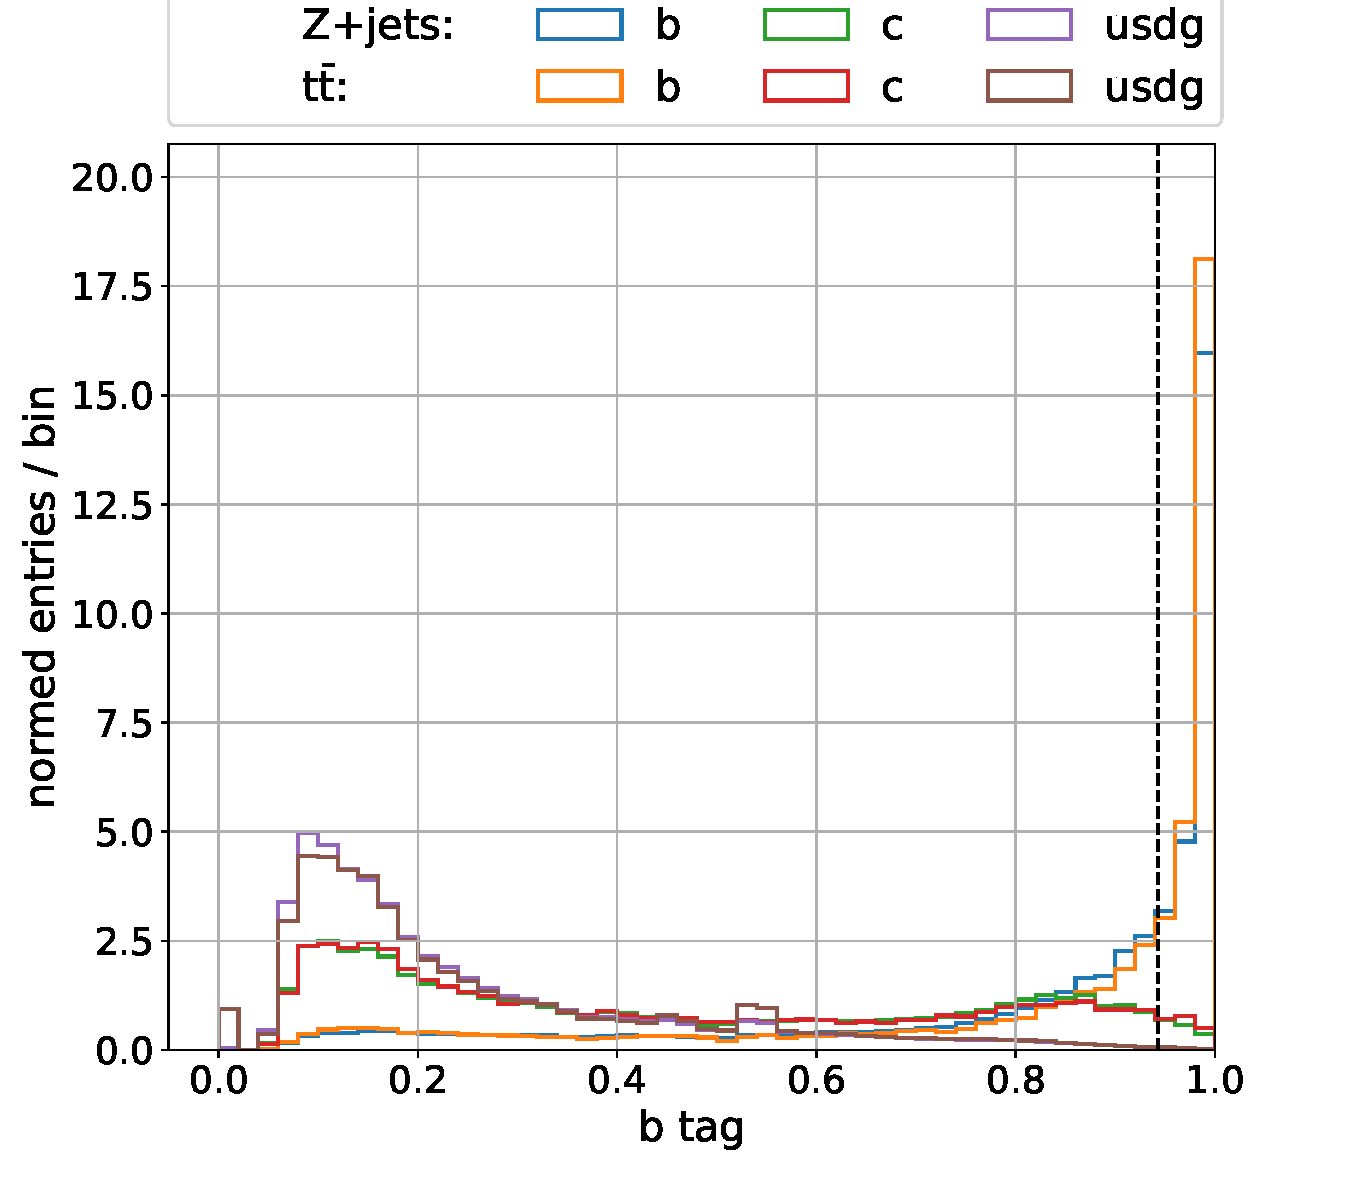
\includegraphics[width=0.45\textwidth]{chapters/Appendix/sectionBtag/figures/bmva_mc.pdf}
    \caption{Distribution of ``bmva" b tagging discriminator for the
    three flavor categories under consideration for Z + jet and
    \ttbar events (left).      
    \label{fig:btag_bmva}}
\end{figure}

\begin{figure}[h!]
    \centering
    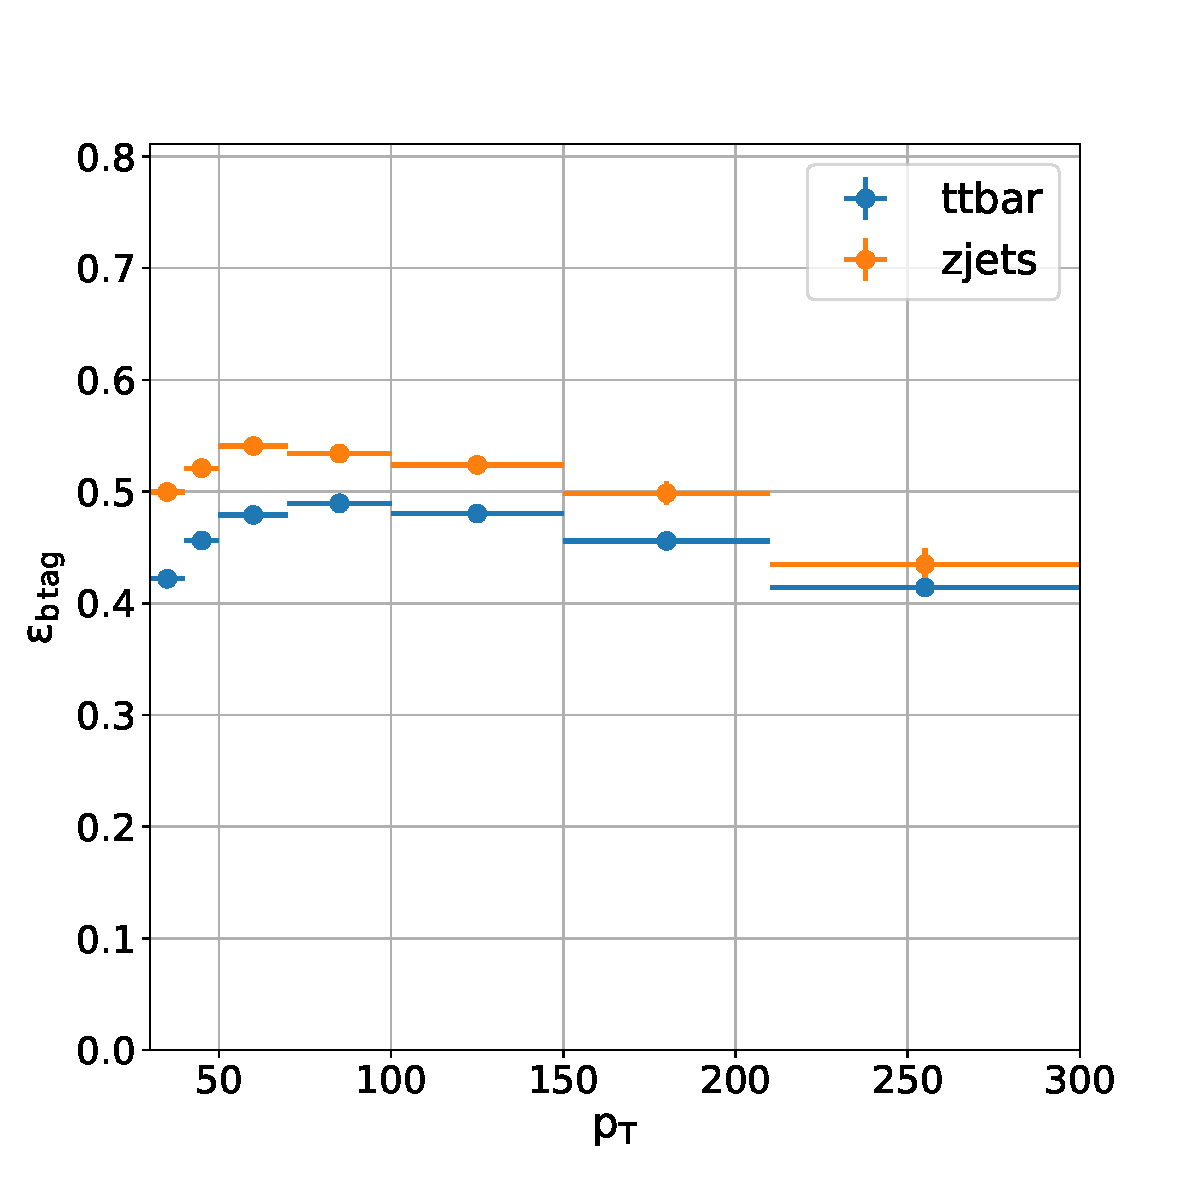
\includegraphics[width=0.3\textwidth]{chapters/Appendix/sectionBtag/figures/bmva_mceff_vs_pt_b}
    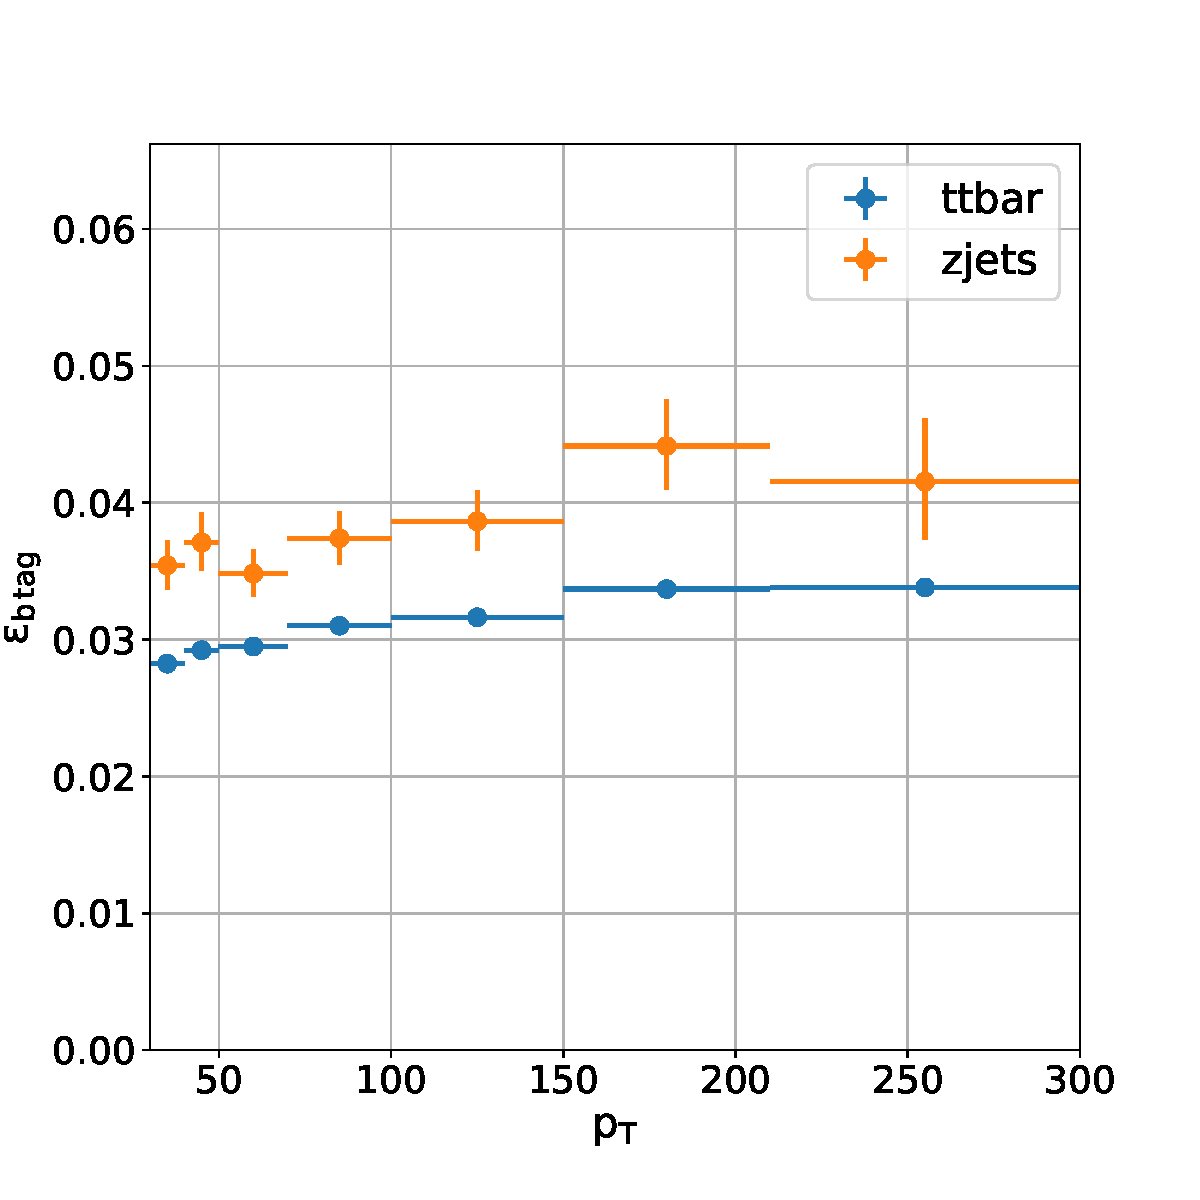
\includegraphics[width=0.3\textwidth]{chapters/Appendix/sectionBtag/figures/bmva_mceff_vs_pt_c}
    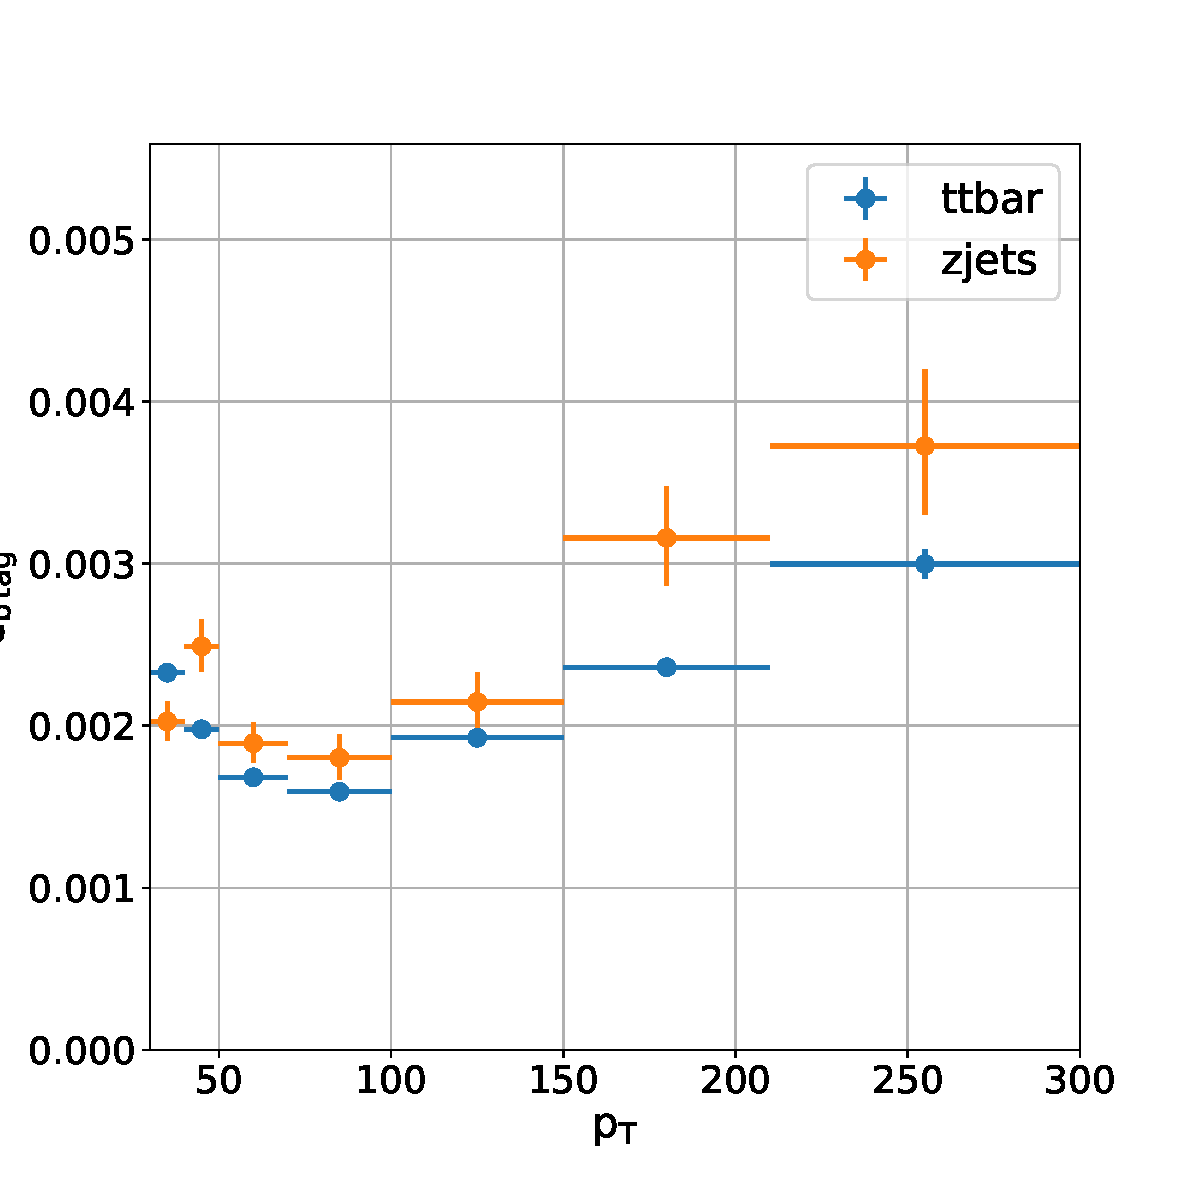
\includegraphics[width=0.3\textwidth]{chapters/Appendix/sectionBtag/figures/bmva_mceff_vs_pt_usdg}
    \caption{Efficiency to b tag a jet originating from a b quark
    \label{fig:btag_eff}
    }
\end{figure}

\FloatBarrier

